\documentclass[12pt]{article}
\usepackage[utf8]{inputenc}
\usepackage{amsmath}
\usepackage{algorithm}
\usepackage{graphicx}
\graphicspath{ {images/} }
\usepackage{hyperref}
\usepackage{amsmath}

\usepackage{algorithm}
\usepackage{algorithmicx}
\usepackage{algpseudocode}

\usepackage{listings}
\usepackage{xcolor}
\usepackage{textcomp}
\usepackage{amssymb}
\usepackage{url}

\usepackage[framed,numbered,autolinebreaks,useliterate]{mcode}


\title{ENGN4528/6528 Computer Vision – 2015 Computer-Lab 4 (C-Lab4)}
\author{Sai Ma - u5224340}
\date{May 2015}

\floatname{algorithm}{Algorithm}
\renewcommand{\algorithmicrequire}{\textbf{input:}}
\renewcommand{\algorithmicensure}{\textbf{output:}}

\begin{document}

\maketitle


\section{Task-1: Implement K-means Clustering Function}
In the first task, it asked us to implement K-means clustering algorithm and providing some existing codes. The implemented code would be used to test two images named \textit{Peppers.png} and \textit{mandm.png}. The more important thing is that assignment asked us to make sure each image is $24$ bits RGB images. Then, we could use Matlab method \textit{uint8} to make sure each layer of given image is $8$ bits, and total image is $24$ bits.

\begin{lstlisting}
Img = imread(ImgName);
Img = uint8(Img);
\end{lstlisting}

\subsection{Extract Vectors}

In the method, we extract feature vectors with $5$ dimensions include a pixel $L$, $a$, $b$ color space values its coordinates values. Therefore, the first sub-task is to extract each pixel feature vector. Then, we could transform RGB image to LAB color space, and add coordinate of each pixel to its vectors. The following is how to implement this process:

\begin{lstlisting}
cform   =  makecform('srgb2lab');
lab = applycform(Img, cform); % get lab value space

% build 5-dimensional feature vectors
features = im2feature(lab, factor, normFlag);
\end{lstlisting}

\begin{lstlisting}
function [ features ] = im2feature( img, factor, normFlag )
% This method used to extract features from given image, becuase this used
% to image segement, then each pixel should have a feature

    [rows, cols, ~] = size(img);
    npixels = rows * cols; % number of pixels

    % Each feature vector consists of [ L,a,b,x,y]
    [x,y] = meshgrid(1:cols, 1:rows); % get x, y values
    
    features = img;
    
    % add two dimensions for x, y coordinates in vectors
    features(:, :, 4) =  factor * x;
    features(:, :, 5) =  factor * y;
    
    features = reshape(features, [npixels 5]);
    features = double(features);
    
    if normFlag > 0
        
        disp('Normalize Features');
        pause(0.03);
        
        % Normalize the features, which benefits to get two vector distance
        for i = 1 : size(features,2)

            MaxValue = max(features(:, i));
            MinValue = min(features(:, i));

            gap = MaxValue - MinValue;

            features(:, i) = (features(:, i) - MinValue) / (gap + eps);

        end
        
    end

end
\end{lstlisting}

Notes that, the normalize process is a signal important pre-process for clustering, because it can ignore the range difference between different dimensions of a vector, and make calculated distance is accurate. For example, three vectors are: a = $[1, 2, 3, 500]$,  b = $[1, 2, 3, 100]$, c =  $[-1, -2, -3, 400]$. Once we did not perform normalized, the first three dimension will make tiny contribute to calculate distance between two vectors, and it will have influence on clustering results. Therefore, the normalized method aims to change these dimensions to same value ranges and make these dimensions weighted same in distance. 

\subsection{Implement K-means Function}

The next job is to implement K-means clustering based on these extracted feature vectors. In the given codes (I changed some argument name to make its name definition clearer), it provides $nFeatures$ to define feature vector number, $ndims$ to represent to vector dimension (in the La*b*, it is $5$), $random_labels$ means the start condition on assign these features to class randomly, $cluster_stats$ defines clustering result (its size is $6$, first index number is the features number belong to this class, and next $5$ numbers are \textit{mean} values of assigned feature vectors), $data_clusters$ saves relationship between feature number and its assigned class number. The most important argument is $distances$ (I change it size to make it can used in my K-means version), it saved all distances information between each feature to all class \textit{mean}. I will explain how to use $distances$ in assignment feature to class in code comments.

In general, the K-means approach includes select start clustering result randomly, calculate \textit{mean} of each class, calculate distances between each vector to each class, and assign this vector to the class with smallest distance to it. The existing code has first and second steps, and also include convergence condition. The other part are include in the following code:

\begin{lstlisting}
function [data_clusters, cluster_stats] = my_kmeans( features, k )

% This function performs k-means clustering on data ,   
% given (k) = the number of clusters.

%  Random Initialization
nFeatures = size(features, 1);
ndims = size(features, 2); % in the L a*b*, it is 5

% in this method, we random assign each feature to a cluster
random_labels = floor(rand(nFeatures, 1) * k) + 1;
% display(random_labels);
data_clusters = random_labels;
cluster_stats = zeros(k, ndims + 1); % centre of clusters
distances = zeros(nFeatures, k);

while(1)
    
    pause(0.03);
    
    % Make a copy of cluster statistics for comparison purposes.  
    % If the difference is very small, the while loop will exit.
    last_clusters = cluster_stats;
    
    % For each cluster    
    for c = 1 : k
        
        % Find all data points assigned to this cluster
        [ind] = find(data_clusters == c);
        
        num_assigned = size(ind, 1);
        
        % some heuristic codes for exception handling. 
        if( num_assigned < 1 )
            disp('No points were assigned to this cluster, some special processing is given below');
            % Calculate the maximum distances from each cluster
            max_distances = max(distances);
            [maxx, cluster_num] = max(max_distances);
            [maxx, data_point] = max(distances(:, cluster_num));
            data_clusters(data_point) = cluster_num;
            ind = data_point;
            num_assigned = 1;
            
        end   %% end of exception handling.   
        % Save number of points per cluster,  plus the mean vectors.
        cluster_stats(c, 1) = num_assigned;
        
        % update centres of clusters
        if( num_assigned > 1 )
            
            summ = sum(features(ind, :));
            cluster_stats(c,2:ndims + 1) = summ / num_assigned;
            
        else
            cluster_stats(c,2:ndims + 1) = features(ind, :);
        end
    end
    
    % Exit criteria
    diff = sum(abs(cluster_stats(:) - last_clusters(:)));
    
    if( diff < 0.00001 )
        break;
    end
    
    % - Set each cluster center to the average of the points assigned to it.
    % - Assign each point to the nearest cluster center  
 
    % first, get distances
    distances = getDistance(cluster_stats, features, ndims);
    
    % then, get smallest distance cluster number, and update the 
    % membership assignment, i.e., update the data_clusters with current values.  
    for featureCount = 1 : 	nFeatures
            
        [~, cluster_num] = min(distances(featureCount,:));
        % cluster_num is class number which has smallest distance to this
        % feature
        data_clusters(featureCount) = cluster_num;
        
    end
    % Display clusters for the purpose of debugging.  
    cluster_stats
    %pause;
 end 
\end{lstlisting}

In the distance calculated approach, I selected squared Euclidean distance. 
\begin{lstlisting}
function [ distances ] = getDistance( cluster_stats, features, ndims )
% This method used to calucate distance between each feature to each
% clusters, then save these reuslts in a distances matrix, which size is
% Number of Feature * Number of Cluster.

% In order to save cacluated process, we use squared Euclidean distance.
    
    k = size(cluster_stats, 1);
    nFeatures = size(features, 1);
    distances = zeros(nFeatures, k);
    
    for featureCount = 1 : nFeatures
        for culsterCount = 1 : k    
            sumDistance = 0;
            for dimCount = 1 : ndims       
                distance = (features(featureCount, dimCount) - cluster_stats(culsterCount, dimCount + 1))^2;
                sumDistance = sumDistance + distance;           
            end
            distances(featureCount, culsterCount) = sqrt(sumDistance);
        end
    end
end
\end{lstlisting}

After get these clustering result, I apply given method \textit{displayclusters} to display clustering result.

\subsection{Implement Clustering Results}

In the K-means algorithm, I set $k$ value to $10$, which means output more colorful. As assignment ask, I changed $factor$ from $1$, $10$ and $20$ display different results \ref{fig:manmFactor1} \ref{fig:manmFactor10} \ref{fig:manmFactor20} \ref{fig:peppersFactor1} \ref{fig:peppersFactor10} \ref{fig:peppersFactor20}.

\begin{figure}[h]
    \centering
    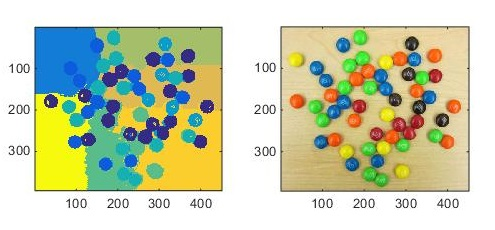
\includegraphics[width=1\textwidth]{manmFactor1.jpg}
    \caption{M \& M with Factor is 1}
    \label{fig:manmFactor1}
\end{figure}

%\begin{figure}[h]
%    \centering
%    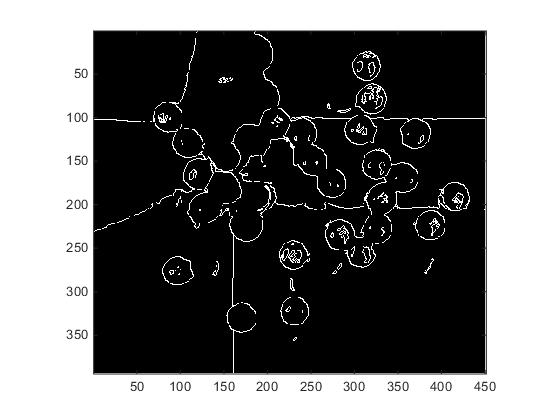
\includegraphics[width=1\textwidth]{manmFactor1boundary.jpg}
%    \caption{M \& M Boundary Image Factor is 1}
%    \label{fig:manmBoundaryFactor1}
%\end{figure}

\begin{figure}[h]
    \centering
    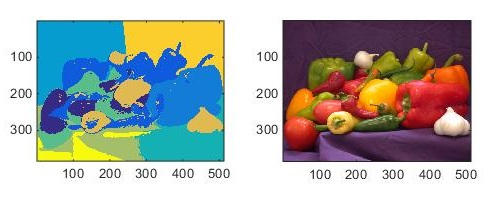
\includegraphics[width=1\textwidth]{peppersFactor1New.jpg}
    \caption{Peppers with Factor is 1}
    \label{fig:peppersFactor1}
\end{figure}

%\begin{figure}[h]
%    \centering
%    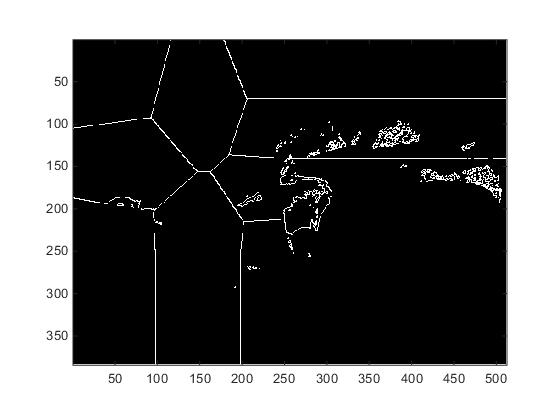
\includegraphics[width=1\textwidth]{peppersFactor1boundary.jpg}
%    \caption{Peppers Boundary Image Factor is 1}
%    \label{fig:pepperBoundaryFactor1}
%\end{figure}

\begin{figure}[h]
    \centering
    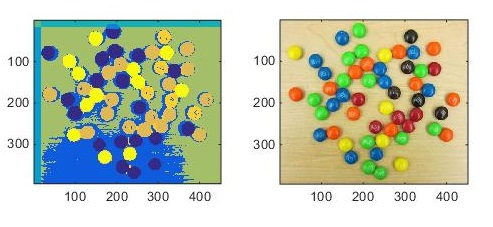
\includegraphics[width=1\textwidth]{manmFactor10.jpg}
    \caption{M \& M with Factor is 10}
    \label{fig:manmFactor10}
\end{figure}

%\begin{figure}[h]
%    \centering
%    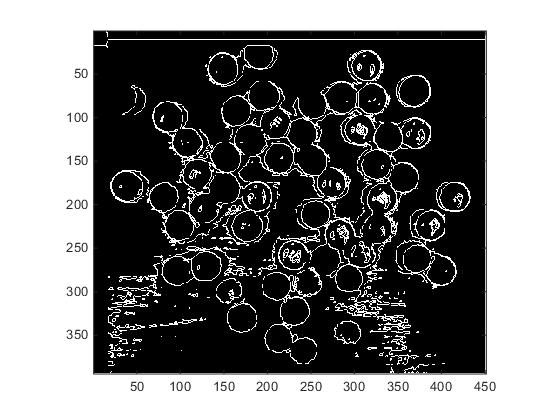
\includegraphics[width=1\textwidth]{manmFactor10boundary.jpg}
%    \caption{M \& M Boundary Image Factor is 10}
%    \label{fig:manmBoundaryFactor10}
%\end{figure}

\begin{figure}[h]
    \centering
    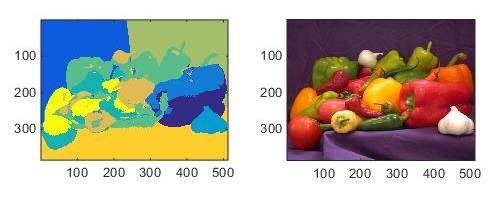
\includegraphics[width=1\textwidth]{peppersFactor10New.jpg}
    \caption{Peppers with Factor is 10}
    \label{fig:peppersFactor10}
\end{figure}

%\begin{figure}[h]
%    \centering
%    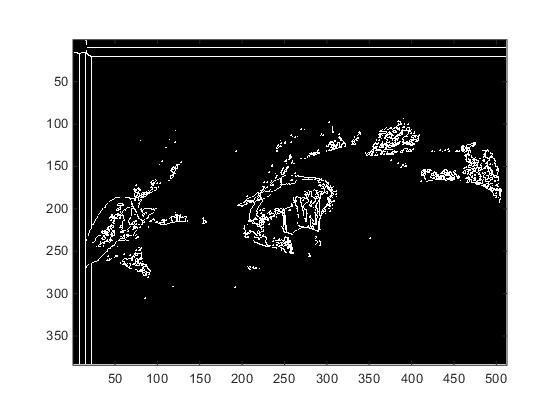
\includegraphics[width=1\textwidth]{peppersFactor10boundary.jpg}
%    \caption{Peppers Boundary Image Factor is 10}
%    \label{fig:pepperBoundaryFactor10}
%\end{figure}


\begin{figure}[h]
    \centering
    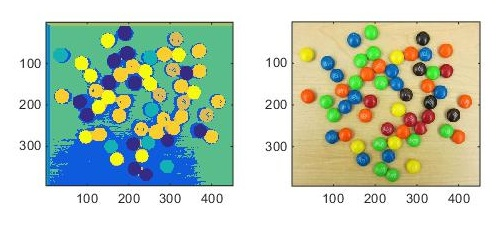
\includegraphics[width=1\textwidth]{manmFactor20.jpg}
    \caption{M \& M with Factor is 20}
    \label{fig:manmFactor20}
\end{figure}

%\begin{figure}[h]
%    \centering
%    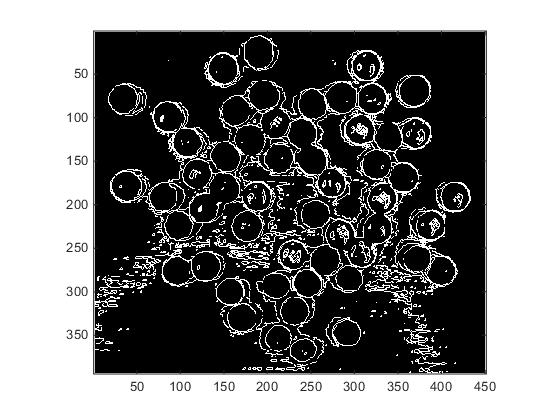
\includegraphics[width=1\textwidth]{manmFactor100boundary.jpg}
%    \caption{M \& M Boundary Image Factor is 100}
%    \label{fig:manmBoundaryFactor100}
%\end{figure}

\begin{figure}[h]
    \centering
    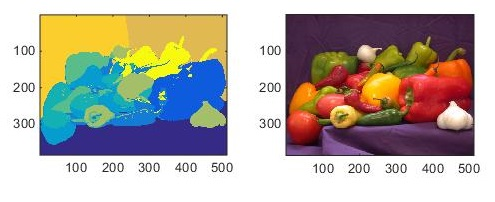
\includegraphics[width=1\textwidth]{peppersFactor20New.jpg}
    \caption{Peppers with Factor is 20}
    \label{fig:peppersFactor20}
\end{figure}

%\begin{figure}[h]
%    \centering
%    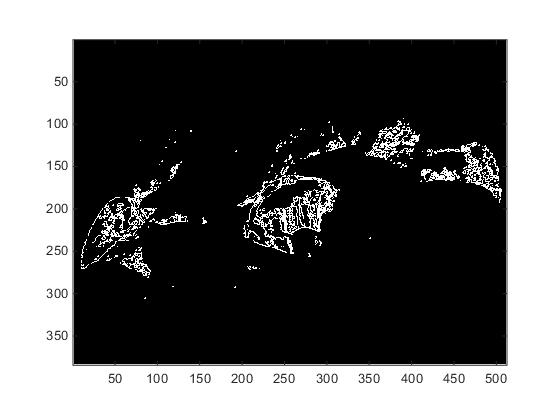
\includegraphics[width=1\textwidth]{peppersFactor100boundary.jpg}
%    \caption{Peppers Boundary Image Factor is 100}
%    \label{fig:pepperBoundaryFactor100}
%\end{figure}

The different values of argument $factor$ cause three different displayed results. The less factor cause clustering result background (empty part) have many clearly segmentation. The reason is that in our implement, the value were saved in \textit{uint8} data format, which value range from $0$ to $255$. The factor used to times coordinates of each feature vector, and make the values are bigger than before. Once we have a bigger $factor$, more values in last two dimensions will be set as maximum. For instance, when we use $10$ to multiply original x value $30$, it will become $255$ in uint8 data format. Then, factor make many vector has same x, y coordinate values, and reduce the weighted of coordinated in clustering. As a result, in these displayed results above, the color difference effect on segmentation result when we have a bigger factor value.

\subsection{Initial Assignment of the K Centers}

In the \textit{K-means} clustering algorithm, it aims to minimize the variance in data given clusters. In the other words, each feature will be calculated the distance between it and cluster centers, and then assign this feature it its nearest (smallest distance) cluster centers. Therefore, we should have the initial K centers, and apply them to compute distances with each features. For example, when we random features (they define the initial cluster centers) did not select well (too close), the finial clustering result will be bad. The following two figures \ref{fig:initialExample1} and \ref{fig:initialExample2} can display how the initial points (initial centers) can effect on cluster result.

\begin{figure}[h]
    \centering
    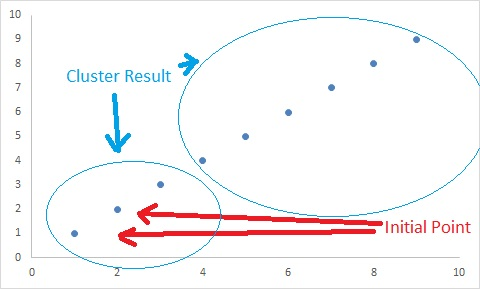
\includegraphics[width=1\textwidth]{initialExample1.jpg}
    \caption{Initial Centers Exampel 1}
    \label{fig:initialExample1}
\end{figure}

\begin{figure}[h]
    \centering
    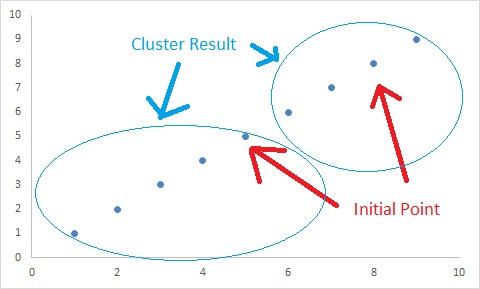
\includegraphics[width=1\textwidth]{initialExample2.jpg}
    \caption{Initial Centers Exampel 2}
    \label{fig:initialExample2}
\end{figure}

In the K-mean method write by my self, I use the codes to initial:

\begin{lstlisting}
% in this method, we random assign each feature to a cluster
random_labels = floor(rand(nFeatures, 1) * k) + 1;
data_clusters = random_labels;
\end{lstlisting}

In the normal K-means approach, we usually select $k$ features randomly, and assign them to $k$ kinds of clusters. Then, at initial situation, each cluster will have one feature. In this K-means, we perform a different approach. For each features, we select one of $k$ cluster randomly, and assign this feature to the random cluster. After assigned all features, we compute the cluster centers. This approach avoid the problem we displayed above because the initial cluster centers will located \textit{far} from others. Then, the clustering result will be better.

\subsection{Key Steps of K-means Clustering Algorithm}

In the K-means algorithm, it includes the key steps on:

\begin{itemize}
  \item 1) Choose $k$, initialize cluster centers
  \item 2) Assign each feature to its closest center
  \item 3) Update the cluster center as the mean points  
  \item 4) Repeat $2$ and $3$ step until clustering result is converged 
\end{itemize}

If we write it in pseudocode (based on my initial approach discussed above) algorithm \ref{alg:kmeans} and algorithm \ref{alg:getCenter}.

\begin{algorithm}
	\caption{K-means}
	\label{alg:kmeans}
	\begin{algorithmic}[1]
	\Require $k$, \textit{features)}
	\Ensure $\{cluster_{1},...cluster_{k}\}$
	\Function{K-means}{$k, features$}
	
	\For{$feature$ in $features$}
		
		\State $i = random(1, k)$
		\State $cluster_{i} \gets feature$
	
	\EndFor	
	
	\For{$cluster_{i}$ in from $cluster_{1}$ to $cluster_{k}$}
		\State $clusterCenter_{i} = getClusterCenter(cluster_{i})$	
	\EndFor	
	
	\While{No Re-assign Features}

		\For{$feature$ in $features$}
			\State $i = argmin(distance(feature, cluster_{1}),... distance(feature, cluster_{k}))$
			\State $cluster_{i} \gets feature$
		\EndFor	
		
		\For{$cluster_{i}$ in $cluster_{1}$ to $cluster_{k}$}
			\State $clusterCenter_{i} = getClusterCenter(cluster_{i})$	
		\EndFor	
	
	\EndWhile

	\State \Return {$\{cluster_{i}, ... cluster{k}\}$}
	
	\EndFunction
	\end{algorithmic}

\end{algorithm}

\begin{algorithm}
	\caption{getClusterCenter}
	\label{alg:getCenter}
	\begin{algorithmic}[1]
	\Require $cluster_{i}$
	\Ensure $clusterCenter_{i}$
	\Function{SIFT}{$cluster_{i}$}
	\State $cluster_{i}$ has assigned $features$
	\State $n$ is number of $features$
	\State $m$ is the dimension of each $feature$

	\For{$c$ in $[1, m]$}

		\State $clusterCenter_{c} = \sum_{1, n}(feature_{c})\times\dfrac{1}{n}$	
	
	\EndFor	
	
	\State \Return{$clusterCenter$}
	\EndFunction
	
	\end{algorithmic}
\end{algorithm}

\subsection{Key Steps of Mean-shift Clustering Algorithm}

In the mean-shift clustering, it aims to segment clustering by the color distribution space. Its main task is to find the \textit{peaks} in the density distribution. Its main tasks are:

\begin{itemize}
  \item 1) Convert image into feature space (based on color density)
  \item 2) Set a fix size search windows distributed over feature space
  \item 3) Compute MEANs of data within each windows  
  \item 4) Sift windows based on computed MEANs above
  \item 5) Repeat step 4 until all windows not moved
\end{itemize}

In the processes, $MEAN$ is the difference between weighted mean of neighbors $xi$ around $x$ and the current value of $x$. 

\section{Task-2: Implement DLT Based Homograph Estimation}

The next task is to build a method to explore \textit{DLT} for homography estimation. As we known, in order to implement \textit{Direct Linear Transforms} approach, we need $4$ or more pairs of points to estimate the $3 \times 3$ homography matrix. In the assignment, it asked us to input $6$ pairs of points to estimate the homography matrix. As a result, the first job is to get $6$ pairs of points. I used Matlab \textit{ginput($12$)} ($12$ means this method will get $12$ points locations). Before run \textit{ginput}, the images $left$ and $right$ should be displayed on screen. Then, the approach to get $6$ pairs of points locations can write in Matlab as following:

\begin{lstlisting}
imgLeft = imread('Left.jpg');
imgRight = imread('Right.jpg');

figure('name', 'Left Image and Right Image');
subplot(1,2,1);
imshow(imgLeft), title('Left Image');
subplot(1,2,2);
imshow(imgRight), title('Right Image');

hold on

% select 6 pairs points from left and right images, left iamge first
[x, y] = ginput(12);
\end{lstlisting}

After these codes, the $6$ pairs of points locations will saved in the argument $[x, y]$. In the assignment, the \textit{DLT} method has $4$ input arguments, and they are $u2Trans$, $v2Trans$, $uBase$, and $vBase$. According to its name definitions, we can easily know that they are the $6$ pairs of points y-scale and x-scale values lists. In the process to get these points, we input $left$ image point firstly. Therefore, we assume that points in the $left$ are $u2Trans$ and $v2Trans$. Then, the next code are how to divided $[y, x]$ to these four input arguments of \textit{DLT}.

\begin{lstlisting}
% get 6 left points from selected points
u2Trans = y(1:2:end,:)'; % odd matrix
v2Trans = x(1:2:end,:)'; % odd matrix

% get 6 right points from selected points
uBase = y(2:2:end,:)'; % even matrix
vBase = x(2:2:end,:)'; % even matrix
\end{lstlisting}

After that, we prepare these input arguments well. I continue to transform these input \textit{DLT} method. According to definition, $(uBase, vBase, 1)'=H*(u2Trans , v2Trans, 1)' $ in this method, and we aims to get $H$. From knowledge on lecture, the $H$ is eigenvector of $A^{T}A$ with smallest eigenvalue. Therefore, in the direct linear transform approach, its main task is to construct $A$. According to its definition, the $A$ matrix is following \ref{A}

\label{A}
$\begin{bmatrix}
x_{1} & y_{1} & 1 & 0 & 0 & 0 & -x'_{1}x_{1} & -x'_{1}y_{1} & -x'_{1}\\ 
0 & 0 & 0 & x_{1} & y_{1} & 1 & -y'_{1}x_{1} & -y'_{1}y_{1} & -y'_{1}\\ 
... \\
x_{n} & y_{n} & 1 & 0 & 0 & 0 & -x'_{n}x_{n} & -x'_{n}y_{n} & -x'_{n}\\ 
0 & 0 & 0 & x_{n} & y_{n} & 1 & -y'_{n}x_{n} & -y'_{n}y_{n} & -y'_{n}
\end{bmatrix}
$

Consider we have $6$ pairs of points, these $n$ is equal to $6$. Then, we should construct this matrix $A$ as its definition. Based on the definition, $u2Trans$ is $x$, $v2Trans$ is $y$, $uBase$ is $x'$ and $vBase$ is $y'$. Then the following is how to construct matrix $A$:

\begin{lstlisting}
% get the vector size, consider of these four arguments have same size,
    % the sizes all are 6
    [pointNums, ~] = size(u2Trans);
    
    % then, consturct matrix A
    A = zeros(2*pointNums, 9);
    
    for count = 1 : pointNums
        
        xPrime = uBase(:, count);
        yPrime = vBase(:, count);
        
        x = u2Trans(:, count);
        y = v2Trans(:, count);
        
        A(2*count - 1,1:9) = [x, y, ones(1, 1), zeros(1, 3), -xPrime*x, -xPrime*y, -xPrime];
        A(2*count, 1:9) = [zeros(1, 3), x, y, ones(1, 1), -yPrime*x, -yPrime*y, -yPrime];
        
    end
\end{lstlisting}

After that, we perform Matlab method \textit{svd} to get its eigenvector with smallest eigenvalue.

\begin{lstlisting}
[~, ~, V] = svd(A);
H = V(:, end); % get the smallest eigenvalue mapped eigenvector
H = reshape(H, 3, 3)'; % change it shape to make used to test solution
leftDown = H(3, 3)';
H = H/leftDown; % make the left down equals to 1
\end{lstlisting}

\subsection{Normalize Points}

However, it we use this $H$ to test whether it is correct $H$, it will not pass. The reason is that we input $6$ pairs of coordinates, and we should normalize the $ubase, vbase, uTrans and vTrans$ values to minimize sum of squared residuals and get the accurate $H$. The following is method on normalize.

\begin{lstlisting}
function [ Points, Transform ] = getNormalize( xValues, yValues )
% get normalize transform for given coorderinates
    
    [~, pointsSize] = size(xValues);
    
    Points = ones(3, pointsSize);
    Points(1, :) = xValues;
    Points(2, :) = yValues;

    % get the mean of x and y
    xMean = mean(xValues); % get centers
    yMean = mean(yValues);
    xDistance = xValues - xMean;
    yDistance = yValues - yMean;

    % get the scale
    xScale = mean(abs(xDistance));
    yScale = mean(abs(yDistance));

    % construct transform matrix and normalization
    Transform = [1/xScale, 0, -xMean/xScale; 0, 1/yScale, -yMean/yScale; 0, 0, 1];
    
end

\end{lstlisting}

Then, we use these normalized transform to multiply our coordinate values, and get stable $H$.

\begin{lstlisting}
% perform normalize approach
[pointBase, transformBase] = getNormalize(uBase, vBase);
[pointTrans, transformTrans] = getNormalize(u2Trans, v2Trans);

% normalize these points
normBase = transformBase*pointBase;
uBase = normBase(1,:);
vBase = normBase(2,:);

normTrans = transformTrans*pointTrans;
u2Trans = normTrans(1,:);
v2Trans = normTrans(2,:);

% then, get the 3*3 homography matrix between these two images
H = DLT(u2Trans, v2Trans, uBase, vBase);
H = (transformBase\H)*transformTrans;
\end{lstlisting}

\subsection{Test Homograph}

In order to prove our $H$ is correct, I write some code to transform image based on our calculated $H$.

\begin{lstlisting}
tform = projective2d(H');
imageNorm = imwarp(imgRight, tform);

figure('name', 'Transform Right Image by H');
subplot(1,3,1), imshow(imageTransform), title('Transform Without Normalized');
subplot(1,3,2), imshow(imageNorm), title('Transform With Normalized');
subplot(1,3,3), imshow(imgLeft), title('Transformed Left Image');
\end{lstlisting}

\begin{figure}[h]
    \centering
    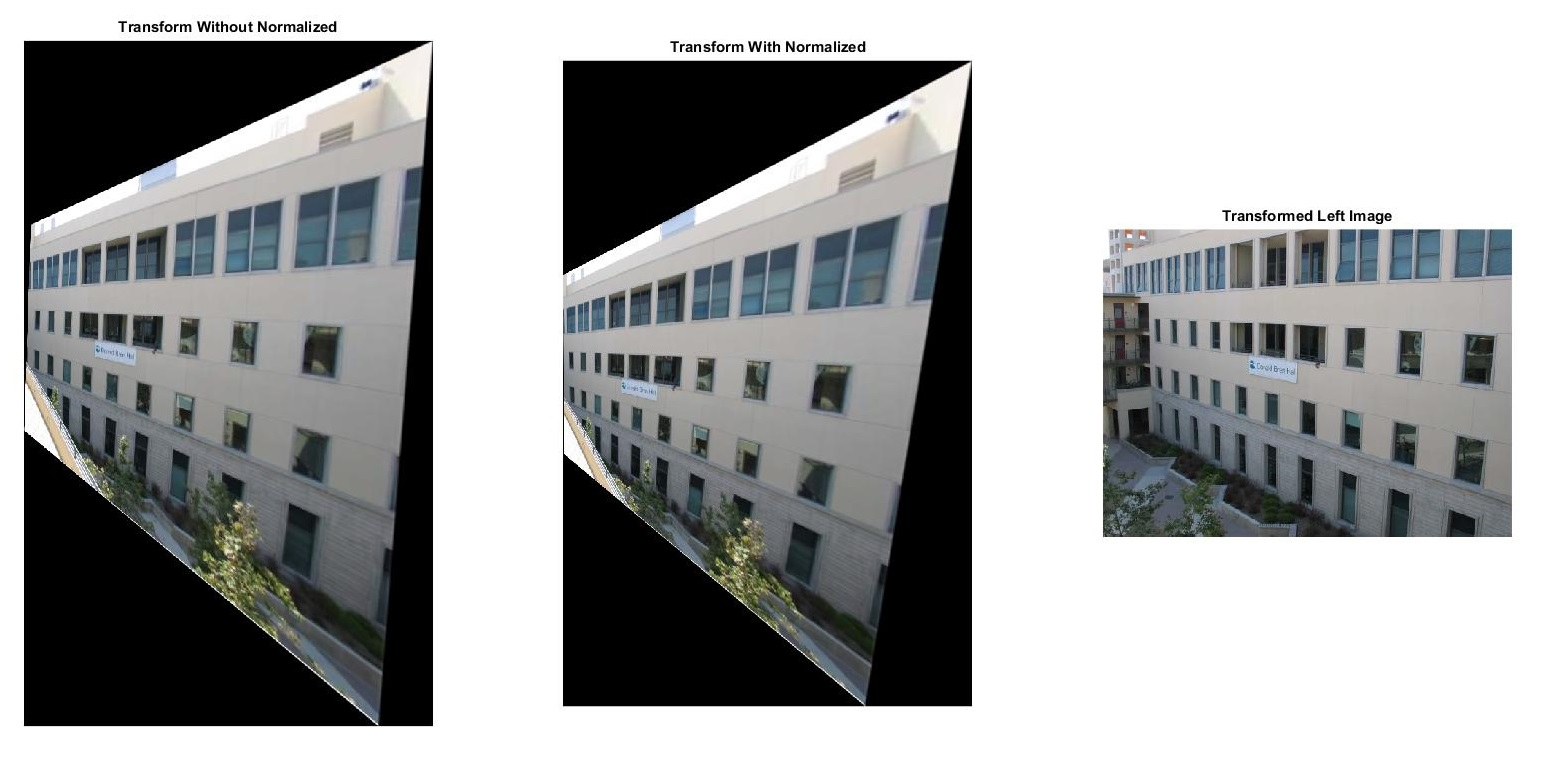
\includegraphics[width=1\textwidth]{TransformResult.jpg}
    \caption{Transformed Result}
    \label{fig:TransformResult}
\end{figure}

After get this figure \ref{fig:TransformResult} above to test $H$, I make sure I get the correct $H$ from my \textit{DLT} method.

\subsection{Linear Equations in Solving Homograph}

In the process of getting homograph, our first task is to get a H that fulfill the equation is:

$\begin{bmatrix} x' \\ y' \\ 1 \end{bmatrix} = \left[ \begin{array}{ccc} h_{00} & h_{01} & h_{02} \\ h_{10} & h_{11} & h_{12} \\ h_{20} & h_{21} & h_{22} \end{array} \right] \times \left[ \begin{array}{c} x \\ y \\ 1 \end{array} \right]$

After expose this equation, we get following equations \ref{eq1}

\begin{equation}
  \begin{aligned}
 		x'_{i}\times(h_{20}\times x_{i} + h_{21}\times y_{i} + h_{22}) = h_{00}\times x_{i} + h_{01}\times y_{i} + h_{02}\\
 		y'_{i}\times(h_{20}\times x_{i} + h_{21}\times y_{i} + h_{22}) = h_{10}\times x_{i} + h_{11}\times y_{i} + h_{12}\\
  \end{aligned}
  \label{eq1}
\end{equation}

Then, the problem become to solve the matrix A eigenvector with its smallest eigenvalue:

$\begin{bmatrix} x_{1} & y_{1} & 1 & 0 & 0 & 0 & -x'_{1}x_{1} & -x'_{1} y_{1} & -x'_{1} \\ 0 & 0 & 0 & x_{1} & y_{1} & 1 &  -y'_{1} x_{1} & -y'_{1} y_{1} & -y'_{1} \\ ...  \\ x_{i} & y_{i} & 1 & 0 & 0 & 0 & -x'_{i}x_{i} & -x'_{i} y_{i} & -x'_{i} \\ 0 & 0 & 0 & x_{i} & y_{i} & 1 &  -y'_{i} x_{i} & -y'_{i} y_{i} & -y'_{i} \end{bmatrix} $

Then, we perform singular value decomposition to get our target $H$.

\subsection{Minimally Points to Compute Homograph}

In the task, we use $6$ pairs of correspondences to compute homograph. In fact, different $4$ pairs of correspondences is enough to compute the homograph. As we analysis before, \textit{projective} degree of freedom is $8$, which means there are $8$ unknown arguments in the transform matrix (because the value at left down of $3 \times 3$ matrix is $1$). For each pair of coordinate, $x'_{i}$ = $\dfrac{h_{00}x_{i}+h_{01}y_{i}+h_{02}}{h_{20}x_{i}+h_{21}y_{i}+h_{22}}$, $y'_{i}$ = $\dfrac{h_{01}x_{i}+h_{11}y_{i}+h_{12}}{h_{20}x_{i}+h_{21}y_{i}+h_{22}}$. In order to solve the $8$ unknown arguments from $h_{00}$ to $h_{21}$ ($h_{22}$ is $1$). We need $4$ pairs of $[x, y]$, $[x',y']$ ($8$ given arguments) to construct polynomial and solve $8$ unknown arguments. 

\section{Appendix: Matlab Code} 
\label{App:AppendixA}

\lstinputlisting{task1.m}
\lstinputlisting{runK_means.m}
\lstinputlisting{displayclusters.m}
\lstinputlisting{task2.m}
\lstinputlisting{DLT.m}

\end{document}